% ═══════════════════════════════════════════════════════════════════════════
%  DFAE  — Descriptor Framework for All Elements
%  NPSPC — Nodal Placement Shape Profile Core
%  HPFC  — High-Performance Flower Compute
%
%  Compile:  pdflatex DFAE.tex  (twice for references)
%            or: latexmk -pdf DFAE.tex
%
%  Part of the FlowerOS HPC stack (docs/DFAE.tex)
% ═══════════════════════════════════════════════════════════════════════════

\documentclass[11pt,a4paper]{article}

% ── packages ──────────────────────────────────────────────────────────────
\usepackage[utf8]{inputenc}
\usepackage[T1]{fontenc}
\usepackage{lmodern}
\usepackage[margin=2.4cm]{geometry}
\usepackage{amsmath,amssymb,amsthm}
\usepackage{graphicx}
\usepackage{xcolor}
\usepackage{booktabs}
\usepackage{enumitem}
\usepackage{hyperref}
\usepackage{tikz}
\usetikzlibrary{arrows.meta,positioning,fit,calc,shapes.geometric}

% ── colours (FlowerOS pastel palette) ────────────────────────────────────
\definecolor{fosMint}{HTML}{87CEEB}
\definecolor{fosMagenta}{HTML}{D8A0D8}
\definecolor{fosGreen}{HTML}{87D687}
\definecolor{fosYellow}{HTML}{F0E68C}
\definecolor{fosGrey}{HTML}{A0A0A0}
\definecolor{fosBlue}{HTML}{6495ED}

\hypersetup{
  colorlinks=true,
  linkcolor=fosBlue,
  citecolor=fosBlue,
  urlcolor=fosMint,
}

% ── theorem-like environments ─────────────────────────────────────────────
\theoremstyle{definition}
\newtheorem{definition}{Definition}[section]
\newtheorem{axiom}[definition]{Axiom}
\newtheorem{contract}[definition]{Contract}
\theoremstyle{plain}
\newtheorem{proposition}[definition]{Proposition}

% ── macros ────────────────────────────────────────────────────────────────
\newcommand{\DFAE}{\textsc{dfae}}
\newcommand{\NPSPC}{\textsc{npspc}}
\newcommand{\HPFC}{\textsc{hpfc}}
\newcommand{\bead}{\boldsymbol{b}}
\newcommand{\desc}{\boldsymbol{d}}
\newcommand{\state}{\boldsymbol{s}}
\newcommand{\shape}{\boldsymbol{g}}
\newcommand{\prov}{\mathcal{P}}
\newcommand{\transfer}{\mathcal{T}}
\newcommand{\constraint}{\mathcal{C}}
\newcommand{\unc}{\sigma}

% ── title ─────────────────────────────────────────────────────────────────
\title{%
  \textbf{DFAE} \\[4pt]
  \Large Descriptor Framework for All Elements \\[14pt]
  \normalsize with \\[6pt]
  \textbf{NPSPC} \quad \large Nodal Placement Shape Profile Core \\[6pt]
  \normalsize and \\[6pt]
  \textbf{HPFC} \quad \large High-Performance Flower Compute%
}
\author{FlowerOS Project}
\date{\today}

% ══════════════════════════════════════════════════════════════════════════
\begin{document}
\maketitle
\thispagestyle{empty}

\begin{abstract}
\noindent
We present the \textbf{Descriptor Framework for All Elements} (\DFAE{}):
a bidirectional multiscale translation-and-constraint architecture
spanning theoretical models, adjacent engineering realisations, and
theoretetically imposed coding frameworks and tools, with
periodic-table generality across chemical, mesoscopic, and continuum
scales.

The local geometry and placement engine that interprets nodal
environments within \DFAE{} is the
\textbf{Nodal Placement Shape Profile Core} (\NPSPC{}):
a lightweight subsystem responsible for form-factor interpretation,
admissible shape logic, and placement profiling, designed to run
on standard 48-core workstation hardware at 150--280~TFlop peak.

The compute infrastructure that executes the full stack is
\textbf{High-Performance Flower Compute} (\HPFC{}):
a customisable operating system division --- built on FlowerOS ---
designed specifically for large-scale descriptor evaluation,
reduction, and systems integration.

\bigskip
\begin{center}
\begin{tabular}{@{}ll@{}}
\toprule
\DFAE{} & defines the cross-scale architecture \\
\NPSPC{} & governs local nodal geometry, placement, and form constraints \\
\HPFC{} & provides the accelerated compute infrastructure that executes the framework \\
\bottomrule
\end{tabular}
\end{center}
\end{abstract}

\tableofcontents
\newpage

% ══════════════════════════════════════════════════════════════════════════
\section{Introduction and Naming}
\label{sec:intro}
% ══════════════════════════════════════════════════════════════════════════

\subsection{Why ``Descriptor Framework for All Elements''?}

\begin{enumerate}[label=(\roman*)]
  \item \textbf{Descriptor} ---
        The framework narrows into a mesoscopic descriptor (bead,
        reduced representation) at the waist; the name foregrounds
        this defining architectural choice.

  \item \textbf{Framework} ---
        ``Framework'' fits better than ``field'' or ``function''
        because the document describes a \emph{bidirectional}
        multiscale translation-and-constraint \emph{system},
        not one isolated method.

  \item \textbf{All Elements} ---
        The scope is periodic-table generality: metals, coordination
        compounds, gases, fluids, and beyond.  The stack spans
        molecular, meso, and engineering realisations across many
        candidate chemistries.
\end{enumerate}

\subsection{Rejected alternatives}

\begin{center}
\begin{tabular}{@{}lll@{}}
\toprule
\textbf{Expansion} & \textbf{Rank} & \textbf{Weakness} \\
\midrule
Descriptor Framework for All Elements  & 1 & --- \\
Descriptor Framework Across Elements   & 2 & Weaker preposition \\
Discrete Framework Across Elements     & 3 & Emphasises discreteness, not
                                               descriptors / contracts / provenance \\
\bottomrule
\end{tabular}
\end{center}

\subsection{Why ``Nodal Placement Shape Profile Core''?}

\NPSPC{} is the local geometry and placement engine that interprets
each node's chemical environment within \DFAE{}.  The name resolves
as follows:

\begin{enumerate}[label=(\roman*)]
  \item \textbf{Nodal} ---
        Each compute node owns and evaluates its own local
        descriptor environment independently; there is no global
        geometry state.

  \item \textbf{Placement} ---
        The subsystem decides where atoms, beads, and coarse-grained
        sites may legitimately reside given the local descriptor and
        the admissible shape set.

  \item \textbf{Shape Profile} ---
        Derived from the VSEPR family of shape logic: the core
        evaluates electron-pair geometry, bond-angle profiles,
        and coordination-environment fingerprints to determine
        the admissible shape set $\mathcal{G}$.

  \item \textbf{Core} ---
        It is a standalone subsystem with a narrow, well-defined
        API; other \DFAE{} modules consume its output but do not
        reach inside it.
\end{enumerate}

\noindent
\textbf{Hardware target:}
Lightweight deployment on a standard 48-core workstation,
150--280~TFlop peak (\emph{typical~48 model for standard parts}).

\subsection{Why ``High-Performance Flower Compute''?}

\HPFC{} is the execution platform.  It is not a library or a
subsystem; it is the \emph{compute division} --- the customisable
operating system layer built on FlowerOS that is designed end-to-end
for this class of task.

\begin{enumerate}[label=(\roman*)]
  \item \textbf{High-Performance} ---
        GPU-first, throughput-oriented; every task executes
        beautifully on accelerated hardware.

  \item \textbf{Flower} ---
        Identity and ecosystem: the name places \HPFC{} inside the
        FlowerOS stack unambiguously and without over-explanation.

  \item \textbf{Compute} ---
        Signals a platform or division, not a single tool ---
        analogous to ``\emph{Apple Silicon},'' not ``\emph{Apple CPU
        library~v3.}''
\end{enumerate}

\begin{center}
\begin{tabular}{@{}lll@{}}
\toprule
\textbf{Expansion} & \textbf{Rank} & \textbf{Note} \\
\midrule
High-Performance Flower Compute   & 1 & Identity + branding; best fit \\
High-Performance Framework Compute & 2 & More institutional, less memorable \\
High-Performance Formation Compute & 3 & Only if formation engine is primary \\
\bottomrule
\end{tabular}
\end{center}

\bigskip
\noindent
\textbf{Polished trio:}
\begin{center}
\begin{tabular}{@{}lp{9cm}@{}}
\toprule
\textbf{\DFAE{}} &
  Introduction to theoretical models which lead to adjacent
  typical engineering, which leads into theoretically imposed
  coding frameworks and tools. \\
\addlinespace
\textbf{\NPSPC{}} &
  Lightweight 150--280~TFlop~PC.  Typical 48-model for standard
  parts.  Local nodal geometry, placement, and shape logic. \\
\addlinespace
\textbf{\HPFC{}} &
  Customisable operating system, designed for this sort of task. \\
\bottomrule
\end{tabular}
\end{center}


% ══════════════════════════════════════════════════════════════════════════
\section{Architectural Overview}
\label{sec:arch}
% ══════════════════════════════════════════════════════════════════════════

\DFAE{} is an hourglass architecture.  Wide at the top (engineering
observables, continuum fields), wide at the bottom (quantum-chemical
all-electron states), and narrow at the \emph{waist}: the mesoscopic
descriptor layer where transferable, reduced representations live.

\begin{center}
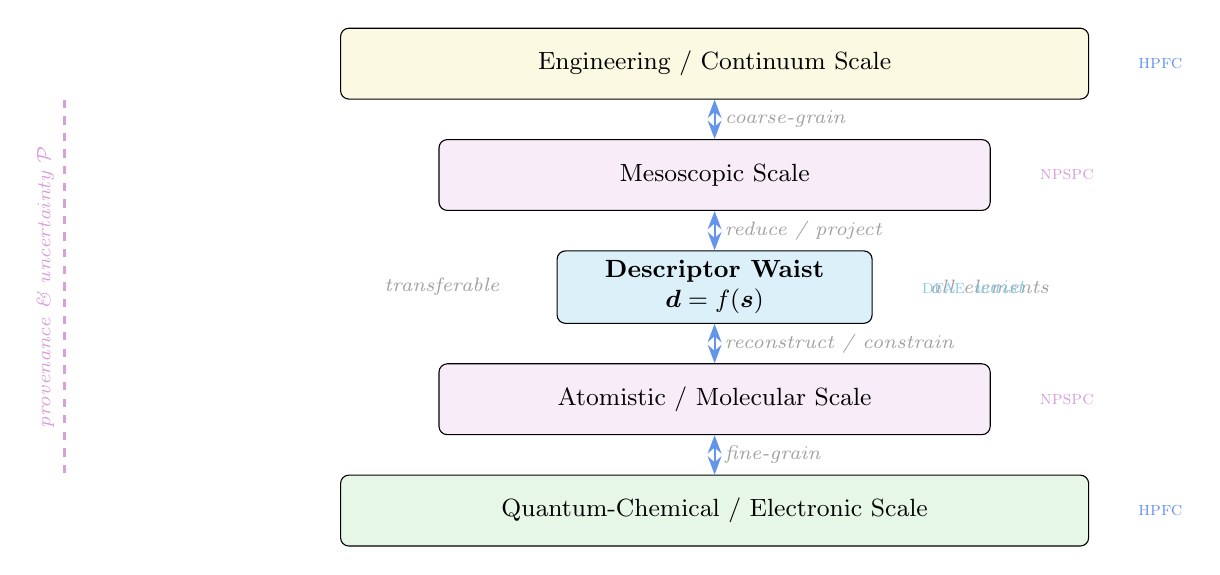
\begin{tikzpicture}[
    >=Stealth,
    layer/.style={draw, rounded corners=3pt, minimum width=#1,
                  minimum height=0.9cm, font=\small, align=center},
    ann/.style={font=\scriptsize\itshape, text=fosGrey},
  ]

  % --- layers (top to bottom) ---
  \node[layer=9.5cm, fill=fosYellow!25]  (eng)
    {Engineering / Continuum Scale};

  \node[layer=7.0cm, fill=fosMagenta!20, below=0.5cm of eng]  (meso)
    {Mesoscopic Scale};

  \node[layer=4.0cm, fill=fosMint!30, below=0.5cm of meso]  (waist)
    {\textbf{Descriptor Waist} \\ $\desc = f(\state)$};

  \node[layer=7.0cm, fill=fosMagenta!20, below=0.5cm of waist]  (atom)
    {Atomistic / Molecular Scale};

  \node[layer=9.5cm, fill=fosGreen!20, below=0.5cm of atom]  (qm)
    {Quantum-Chemical / Electronic Scale};

  % --- arrows ---
  \draw[<->, thick, fosBlue]
    (eng.south) -- node[right, ann]{coarse-grain} (meso.north);
  \draw[<->, thick, fosBlue]
    (meso.south) -- node[right, ann]{reduce / project} (waist.north);
  \draw[<->, thick, fosBlue]
    (waist.south) -- node[right, ann]{reconstruct / constrain} (atom.north);
  \draw[<->, thick, fosBlue]
    (atom.south) -- node[right, ann]{fine-grain} (qm.north);

  % --- annotations ---
  \node[ann, left=0.6cm of waist] {transferable};
  \node[ann, right=0.6cm of waist] {all elements};

  % --- component labels (right margin) ---
  \node[ann, right=0.5cm of eng,  text=fosBlue]    {\HPFC{}};
  \node[ann, right=0.5cm of meso, text=fosMagenta] {\NPSPC{}};
  \node[ann, right=0.5cm of waist,text=fosMint]    {\DFAE{} waist};
  \node[ann, right=0.5cm of atom, text=fosMagenta] {\NPSPC{}};
  \node[ann, right=0.5cm of qm,   text=fosBlue]    {\HPFC{}};

  % --- provenance spine ---
  \draw[dashed, thick, fosMagenta]
    ([xshift=-3.5cm]eng.south west) -- ([xshift=-3.5cm]qm.north west)
    node[midway, left, ann, text=fosMagenta, rotate=90, anchor=south]
    {provenance \& uncertainty $\prov$};

\end{tikzpicture}
\end{center}


% ══════════════════════════════════════════════════════════════════════════
\section{The Descriptor Waist}
\label{sec:waist}
% ══════════════════════════════════════════════════════════════════════════

\begin{definition}[Descriptor]
\label{def:descriptor}
A \emph{descriptor} $\desc \in \mathbb{R}^{D}$ is a reduced
representation of a local chemical environment such that:
\begin{enumerate}[label=(\alph*)]
  \item $\desc$ is \textbf{invariant} to rigid rotation, translation, and
        permutation of like atoms;
  \item the map $\state \mapsto \desc$ is \textbf{smooth} and
        \textbf{differentiable} almost everywhere; and
  \item the map $\desc \mapsto \hat{\state}$ (reconstruction) preserves
        all symmetry-allowed information to within a bounded
        uncertainty $\unc$.
\end{enumerate}
\end{definition}

\begin{definition}[Bead]
A \emph{bead} $\bead$ is the mesoscopic counterpart of a descriptor:
it aggregates a cluster of descriptors into a single super-site with
an effective potential, effective composition, and effective geometry.
Beads are the primitive objects in coarse-grained simulation.
\[
  \bead = \operatorname{Aggregate}\!\bigl(
    \{\desc_i\}_{i \in \text{cluster}}\bigr)
\]
\end{definition}

\noindent
The waist is narrow by design: every upward or downward traversal
of the hourglass must pass through the descriptor layer, enforcing
\emph{information discipline} and enabling transferability across
elements, phases, and length scales.


% ══════════════════════════════════════════════════════════════════════════
\section{Transfer Contracts}
\label{sec:contracts}
% ══════════════════════════════════════════════════════════════════════════

\begin{contract}[Scale-Crossing Transfer]
\label{con:transfer}
A transfer $\transfer_{A \to B}$ from scale~$A$ to scale~$B$ is valid
if and only if:
\begin{enumerate}[label=(\roman*)]
  \item \textbf{Descriptor compatibility:}
        the source descriptor $\desc^{A}$ and target descriptor
        $\desc^{B}$ share a compatible invariant basis;
  \item \textbf{Provenance chain:}
        a complete provenance record $\prov(\transfer)$ traces every
        reduction, projection, and approximation back to the
        originating all-electron state;
  \item \textbf{Uncertainty bound:}
        the propagated uncertainty satisfies
        $\unc(\desc^{B}) \le \unc_{\max}^{B}$; and
  \item \textbf{Constraint satisfaction:}
        all reflective constraints $\constraint$ imposed by the
        target scale are satisfied after the transfer.
\end{enumerate}
\end{contract}

\noindent
Contracts are enforced at runtime by \NPSPC{} (local geometry
validation) and \HPFC{} (execution-layer rejection).  A transfer
that violates any clause is \emph{rejected}, not silently degraded.


% ══════════════════════════════════════════════════════════════════════════
\section{Provenance and Uncertainty}
\label{sec:provenance}
% ══════════════════════════════════════════════════════════════════════════

Provenance is not bolted-on metadata; it is a first-class kernel
object.

\begin{definition}[Provenance Record]
\label{def:prov}
A provenance record $\prov$ is a directed acyclic graph (DAG) whose
nodes are \emph{computational events} (descriptor evaluations,
coarse-graining steps, reconstructions, constraint checks) and whose
edges encode data flow.  Each node carries:
\begin{itemize}[nosep]
  \item An \textbf{event hash} (SHA-256 of inputs + code version);
  \item A \textbf{timestamp} (nanosecond wall-clock);
  \item An \textbf{uncertainty annotation} $\unc$; and
  \item A \textbf{node identity} (which \NPSPC{} / \HPFC{} node executed it).
\end{itemize}
\end{definition}

\begin{axiom}[Monotonic Uncertainty]
\label{ax:uncertainty}
Uncertainty never silently decreases.  If scale~$B$ claims a tighter
bound than scale~$A$ provided, the transfer contract requires an
explicit justification event in the provenance DAG (e.g.\ a Bayesian
update with new data).
\end{axiom}


% ══════════════════════════════════════════════════════════════════════════
\section{Reflective Constraints}
\label{sec:constraints}
% ══════════════════════════════════════════════════════════════════════════

\begin{definition}[Reflective Constraint]
\label{def:constraint}
A \emph{reflective constraint} $\constraint$ is a predicate on
the descriptor space that is imposed by one scale upon another:
\[
  \constraint : \mathbb{R}^{D} \to \{\texttt{true}, \texttt{false}\}
\]
Constraints propagate \emph{bidirectionally}: a coarse-grained model
may constrain the admissible fine-grained reconstructions, and vice
versa.
\end{definition}

\noindent
Examples:
\begin{itemize}[nosep]
  \item \textbf{Stoichiometry lock} ---
        the bead-level composition must be consistent with the
        atomistic partition.
  \item \textbf{Energy consistency} ---
        the coarse-grained free energy must lie within $\unc$ of
        the fine-grained reference.
  \item \textbf{Symmetry inheritance} ---
        if the engineering-scale field has a crystallographic space
        group, the descriptor waist must respect it.
\end{itemize}


% ══════════════════════════════════════════════════════════════════════════
\section{NPSPC: Nodal Placement Shape Profile Core}
\label{sec:npspc}
% ══════════════════════════════════════════════════════════════════════════

\NPSPC{} is the local geometry and placement engine.  It runs on
each compute node and answers one question per site: \emph{what
shapes are admissible here, and where may the next atom or bead
be placed?}

\begin{definition}[Admissible Shape Set]
\label{def:shape}
For a site with descriptor $\desc$, the \emph{admissible shape set}
$\mathcal{G}(\desc)$ is the set of all coordination geometries
consistent with $\desc$ under the active reflective constraints:
\[
  \mathcal{G}(\desc) = \bigl\{\shape \in \mathrm{VSEPR}
    \mid \constraint(\desc, \shape) = \texttt{true}\bigr\}
\]
where $\mathrm{VSEPR}$ denotes the full library of electron-pair
geometries (linear, trigonal, tetrahedral, octahedral, \ldots).
\end{definition}

\subsection{Internal modules}

\begin{center}
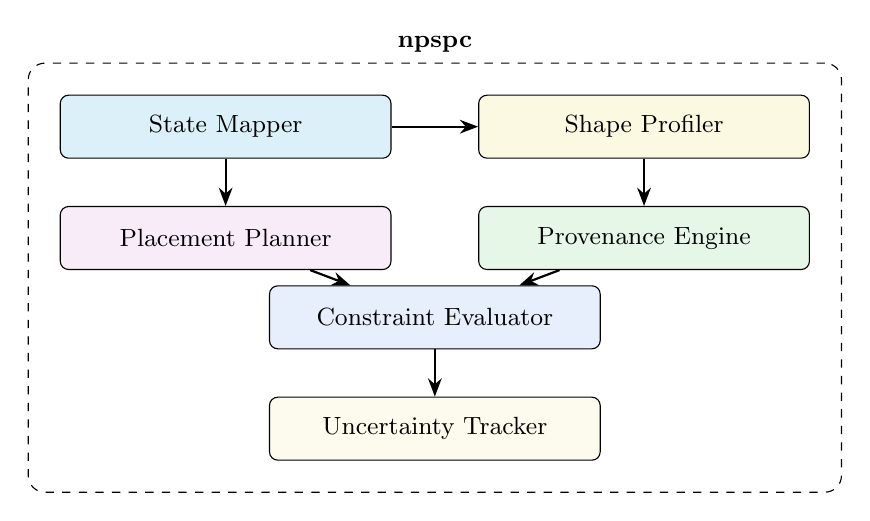
\begin{tikzpicture}[
    >=Stealth,
    mod/.style={draw, rounded corners=3pt, minimum width=4.2cm,
                minimum height=0.8cm, font=\small, align=center},
    ann/.style={font=\scriptsize\itshape, text=fosGrey},
  ]

  \node[mod, fill=fosMint!30]   (sm) {State Mapper};
  \node[mod, fill=fosYellow!25, right=1.1cm of sm] (sp) {Shape Profiler};
  \node[mod, fill=fosMagenta!20, below=0.6cm of sm] (pp) {Placement Planner};
  \node[mod, fill=fosGreen!20,  below=0.6cm of sp] (pe) {Provenance Engine};
  \node[mod, fill=fosBlue!15,  below=0.6cm of $(pp)!0.5!(pe)$] (ce)
    {Constraint Evaluator};
  \node[mod, fill=fosYellow!15, below=0.6cm of ce] (ue) {Uncertainty Tracker};

  \draw[->, thick] (sm) -- (sp);
  \draw[->, thick] (sm) -- (pp);
  \draw[->, thick] (sp) -- (pe);
  \draw[->, thick] (pp) -- (ce);
  \draw[->, thick] (pe) -- (ce);
  \draw[->, thick] (ce) -- (ue);

  \node[draw, dashed, rounded corners=6pt, inner sep=0.4cm,
        fit=(sm)(sp)(pp)(pe)(ce)(ue),
        label={[font=\small\bfseries]above:\NPSPC{}}] {};

\end{tikzpicture}
\end{center}

\begin{center}
\begin{tabular}{@{}lp{8.5cm}@{}}
\toprule
\textbf{Module} & \textbf{Responsibility} \\
\midrule
State Mapper &
  Maps raw simulation state $\state$ to the descriptor $\desc$ and back.
  Owns the forward (reduce) and inverse (reconstruct) transforms. \\[4pt]

Shape Profiler &
  Evaluates the admissible shape set $\mathcal{G}(\desc)$
  (Definition~\ref{def:shape}); classifies electron-pair geometry,
  bond-angle profiles, and coordination fingerprints. \\[4pt]

Placement Planner &
  Given $\mathcal{G}(\desc)$, determines admissible positions for
  the next atom, bead, or coarse-grained site.  Checks
  Contract~\ref{con:transfer} before committing any placement. \\[4pt]

Provenance Engine &
  Maintains the provenance DAG (Definition~\ref{def:prov}).
  Records every shape decision, placement event, and constraint
  check with its event hash and timestamp. \\[4pt]

Constraint Evaluator &
  Checks all active reflective constraints $\constraint$ against
  the current descriptor and shape state.  Propagates violations
  bidirectionally. \\[4pt]

Uncertainty Tracker &
  Enforces Axiom~\ref{ax:uncertainty}.  Propagates and validates
  uncertainty bounds through every placement and reconstruction
  step. \\
\bottomrule
\end{tabular}
\end{center}

\subsection{Hardware target}

\NPSPC{} is deliberately lightweight.  The design point is a
standard 48-core workstation at 150--280~TFlop peak
(``\emph{typical~48 model for standard parts}''): no specialist
hardware required, no dependency on large cluster allocation.
Scaling to \HPFC{}-class hardware is additive, not required.

% ══════════════════════════════════════════════════════════════════════════
\section{HPFC: High-Performance Flower Compute}
\label{sec:hpfc}
% ══════════════════════════════════════════════════════════════════════════

\HPFC{} is the compute division --- the operating system and
execution platform built on FlowerOS that runs \DFAE{} workloads
at scale.  It is not a library or a module; it is a \emph{branded
execution layer}.

\subsection{Role in the stack}

\begin{center}
\begin{tabular}{@{}lp{9cm}@{}}
\toprule
\textbf{Layer} & \textbf{What \HPFC{} provides} \\
\midrule
OS foundation &
  Customisable FlowerOS installation (Tier~1 bare metal or
  Tier~5 Linux power install) tuned for sustained GPU throughput. \\
\addlinespace
Scheduler &
  GPU-first work distribution across \NPSPC{} nodes; batched
  descriptor evaluation; reduction pipelines. \\
\addlinespace
Runtime services &
  Theme-aware terminal, named-pipe IPC bus, persistent state
  store, GPU detect, MOTD, and the full FlowerOS tool suite. \\
\addlinespace
Systems integration &
  Interfaces \DFAE{} transfer contracts with the FlowerOS
  Pollination (IPC) and Thorns (security) subsystems. \\
\bottomrule
\end{tabular}
\end{center}

\subsection{Compute tiers}

\begin{center}
\begin{tabular}{@{}llll@{}}
\toprule
\textbf{Tier} & \textbf{Hardware} & \textbf{Peak} & \textbf{Use case} \\
\midrule
NPSPC node    & 48-core workstation          & 150--280~TFlop & Local NPSPC \\
HPFC entry    & 1--2$\times$ GPU (8--24~GB)  & 300~TFlop+     & Single-node DFAE \\
HPFC standard & 4$\times$ A100 (80~GB each)  & 2~PFlop        & Full DFAE cluster \\
HPFC extended & Multi-node, NVLink           & Unlimited      & Production HPC \\
\bottomrule
\end{tabular}
\end{center}

\subsection{Naming note}

The \emph{Flower} in \HPFC{} is load-bearing: it places the
division inside the FlowerOS ecosystem without qualification.
A future sub-product (e.g.\ \textit{HPFC~Cluster Edition}) inherits
that identity automatically.  The name works as a brand, as an
internal division name, and as a technical label simultaneously ---
which is why the generic alternatives (\emph{Framework Compute},
\emph{Formation Compute}) rank lower.


% ══════════════════════════════════════════════════════════════════════════
\section{Periodic-Table Generality}
\label{sec:elements}
% ══════════════════════════════════════════════════════════════════════════

The ``All Elements'' commitment means the descriptor waist must not
be hard-coded to a single chemistry.  \DFAE{} achieves this through:

\begin{enumerate}[label=\arabic*.]
  \item \textbf{Element-indexed descriptor banks} ---
        each element (or element pair) registers a descriptor
        template; the waist assembles composite descriptors from
        these templates at runtime.

  \item \textbf{Coordination-agnostic invariants} ---
        descriptors are built on smooth, body-ordered invariants
        (e.g.\ \emph{Atomic Cluster Expansion} or
        \emph{Smooth Overlap of Atomic Positions} families) that
        handle arbitrary coordination environments without
        special-case branching.

  \item \textbf{Phase-neutral representation} ---
        the same descriptor algebra covers solids, liquids, gases,
        and interfaces; only the aggregation kernel (bead definition)
        changes.
\end{enumerate}

\noindent
Target chemistry families in the current roadmap:
\begin{center}
\begin{tabular}{@{}ll@{}}
\toprule
\textbf{Family} & \textbf{Representative systems} \\
\midrule
Transition metals           & Fe, Cu, Ni alloys; catalytic surfaces \\
Coordination compounds      & Metal--organic frameworks; ligand fields \\
Light-element covalent      & C, Si, B, N polymorphs; organic molecules \\
Gases and supercritical     & CO$_2$, H$_2$O, N$_2$ at high \emph{P/T} \\
Ionic / molten salts        & NaCl, LiF, rare-earth halides \\
\bottomrule
\end{tabular}
\end{center}


% ══════════════════════════════════════════════════════════════════════════
\section{Integration with FlowerOS HPC}
\label{sec:floweros}
% ══════════════════════════════════════════════════════════════════════════

The three-name hierarchy maps cleanly onto the existing FlowerOS
kernel subsystems defined in \texttt{flower\_kernel.h}:

\begin{center}
\begin{tabular}{@{}llll@{}}
\toprule
\textbf{Component} & \textbf{Module} & \textbf{FlowerOS subsystem} &
  \textbf{Source} \\
\midrule
\NPSPC{} & State Mapper       & Garden (memory)            & \texttt{flower\_kernel.h} \\
\NPSPC{} & Shape Profiler     & Petals (GPU compute)       & \texttt{flower\_kernel.c} \\
\NPSPC{} & Placement Planner  & Pollination (IPC)          & \texttt{flower\_kernel.c} \\
\NPSPC{} & Provenance Engine  & Thorns (security / audit)  & \texttt{flower\_kernel.h} \\
\NPSPC{} & Constraint Eval.   & Photosynthesis (resources) & \texttt{flower\_kernel.c} \\
\NPSPC{} & Uncertainty Tracker& Seeding (entropy)          & \texttt{flower\_kernel.h} \\
\addlinespace
\HPFC{} & Scheduler          & Petals (GPU cores)         & \texttt{flower\_kernel.c} \\
\HPFC{} & IPC bus            & Stem (network stack)       & \texttt{flower\_kernel.h} \\
\HPFC{} & State store        & Tier~4 broker              & \texttt{tier4/broker.c}   \\
\bottomrule
\end{tabular}
\end{center}

\noindent
The Thorns security subsystem (\texttt{flower\_kernel.h}, \S5)
provides per-process capability masks, audit logging, and integrity
verification --- these map directly onto \NPSPC{}'s provenance
enforcement.  The Tier~4 named-pipe broker
(\texttt{tier4/broker.c}) is the natural home for the \HPFC{}
scheduler's inter-node state propagation.


% ══════════════════════════════════════════════════════════════════════════
\section{Formal Summary}
\label{sec:summary}
% ══════════════════════════════════════════════════════════════════════════

\begin{proposition}[Completeness of the naming trio]
The trio $(\textsc{dfae},\;\textsc{npspc},\;\textsc{hpfc})$
is \emph{complete} in the following sense:
\begin{enumerate}[label=(\alph*)]
  \item Every concept in the multiscale stack (descriptors, beads,
        transfers, shape logic, placement, constraints, provenance,
        uncertainty, execution, scheduling) is addressable from
        exactly one of the three names.
  \item \DFAE{} covers \emph{what} is being modelled (the theory
        and cross-scale architecture).
  \item \NPSPC{} covers \emph{where} things go locally (nodal
        geometry, shape, and placement, on lightweight hardware).
  \item \HPFC{} covers \emph{how} it runs at scale (the
        customisable OS and accelerated execution platform).
  \item The three names are mutually non-overlapping: none can
        substitute for another without information loss.
\end{enumerate}
\end{proposition}

\bigskip
\begin{center}
\fbox{\parbox{0.92\linewidth}{\centering
  \textbf{DFAE} --- Descriptor Framework for All Elements \\[4pt]
  \small
  Introduction to theoretical models $\to$ adjacent typical
  engineering $\to$ theoretically imposed coding frameworks and tools.
  \\[8pt]
  \normalsize
  \textbf{NPSPC} --- Nodal Placement Shape Profile Core \\[4pt]
  \small
  Lightweight 150--280~TFlop PC.  Typical 48 model for standard
  parts.  Local nodal geometry, placement, and shape logic.
  \\[8pt]
  \normalsize
  \textbf{HPFC} --- High-Performance Flower Compute \\[4pt]
  \small
  Customisable operating system, designed for this sort of task.
}}
\end{center}

\end{document}
